\section{Introducción}

En el ámbito global, la Inteligencia Artificial (IA) ha revolucionado diversos sectores, facilitando la toma de decisiones, optimizando procesos y generando soluciones innovadoras para problemas complejos. Particularmente, la IA ha demostrado su potencial en la mejora de sistemas de software diseñados para sectores específicos como lo es el sector de la Seguridad y Salud en el Trabajo (SST), especialmente en contextos como el colombiano que se encuentra en la cúspide de esta revolución tecnológica donde organizaciones como la Corporación Talentum aspiran a liderar iniciativas que generen un impacto positivo en el bienestar laboral.

No obstante, emerge una problemática significativa: a pesar de los avances en IA, su integración efectiva en soluciones de software orientadas a la SST presenta desafíos que abarcan desde aspectos técnicos hasta cuestiones éticas y de privacidad, y demandan una comprensión profunda y enfoques adaptados para asegurar implementaciones exitosas que realmente beneficien a los usuarios finales y a las organizaciones involucradas.

Es imperativo abordar esta problemática, dado que las soluciones adecuadas poseen el potencial de transformar cómo las organizaciones gestionan la Seguridad y Salud en el Trabajo. Una implementación efectiva de IA puede facilitar la identificación temprana de riesgos, optimizar respuestas y promover ambientes de trabajo más seguros y saludables. Por lo tanto, resulta esencial establecer estrategias y métodos claros que permitan maximizar los beneficios de la IA en este sector.

En este contexto, se presenta esta propuesta con el propósito de establecer dichas estrategias y métodos para una efectiva incorporación de componentes de IA en soluciones dirigidas al sector mencionado. Con este fin, no solo se plantea el objetivo de proporcionar directrices claras y evidencia palpable de cómo la IA puede enriquecer este campo, sino que también se espera producir resultados concretos: un conjunto de principios arquitectónicos fundamentales para considerar al diseñar software con requisitos relacionados con la IA; un prototipo funcional web y modular que demuestre la aplicación del marco de trabajo documentado; y finalmente, un documento detallado que defina el marco de trabajo y ofrezca buenas prácticas, convenciones y requisitos esenciales para la adecuada integración de aplicaciones con componentes de IA.

Para lograr una comprensión profunda y enfrentar la problemática destacada, se realizará una revisión de literatura, fundamentado en una revisión de documentos existentes, el análisis de datos pertinentes y la aplicación de metodologías apropiadas. De esta manera, se proporcionará no solo una base sólida para futuras implementaciones de IA en el ámbito de SST, sino también en productos que incorporen IA en sus requerimientos funcionales.

La estructura de este documento se ha diseñado para facilitar la comprensión y el análisis de cada aspecto involucrado en la incorporación de la Inteligencia Artificial al sector de la Seguridad y Salud en el Trabajo (SST). Comenzando con una definición del problema en la Sección 2, se elabora sobre la situación actual y las preguntas específicas que guían este estudio. Los Objetivos del proyecto, tanto generales como específicos, así como los resultados esperados, se exponen en la Sección 3, mientras que el Alcance del estudio se detalla en la Sección 4. La justificación del trabajo de grado se presenta en la Sección 5, seguida por el Marco teórico de referencia y antecedentes, que incluye las Bases Teóricas y el Estado del Arte en la Sección 6, proporcionando un contexto esencial para la investigación. La metodología adoptada para llevar a cabo esta investigación se describe en la Sección 7. Los recursos necesarios para la ejecución del proyecto, incluyendo los Recursos Humanos, Bibliográficos y Tecnológicos se enumeran en la Sección 8. Finalmente, la Sección 9 esboza el Cronograma de actividades que guiará el desarrollo de la investigación, seguido por las Referencias Bibliográficas y el Glosario de Términos en las secciones 10 y 11, respectivamente.

Para sintetizar y visualizar la estructura integral de la investigación y sus componentes clave, se presenta la siguiente figura. Este esquema gráfico tiene como objetivo proporcionar una representación clara y concisa de la propuesta de proyecto, destacando cómo cada elemento interactúa y contribuye al desarrollo de soluciones innovadoras y eficaces para la integración de la IA en el sector de la SST.

\begin{figure}[H]
\centering
\rotatebox{90}{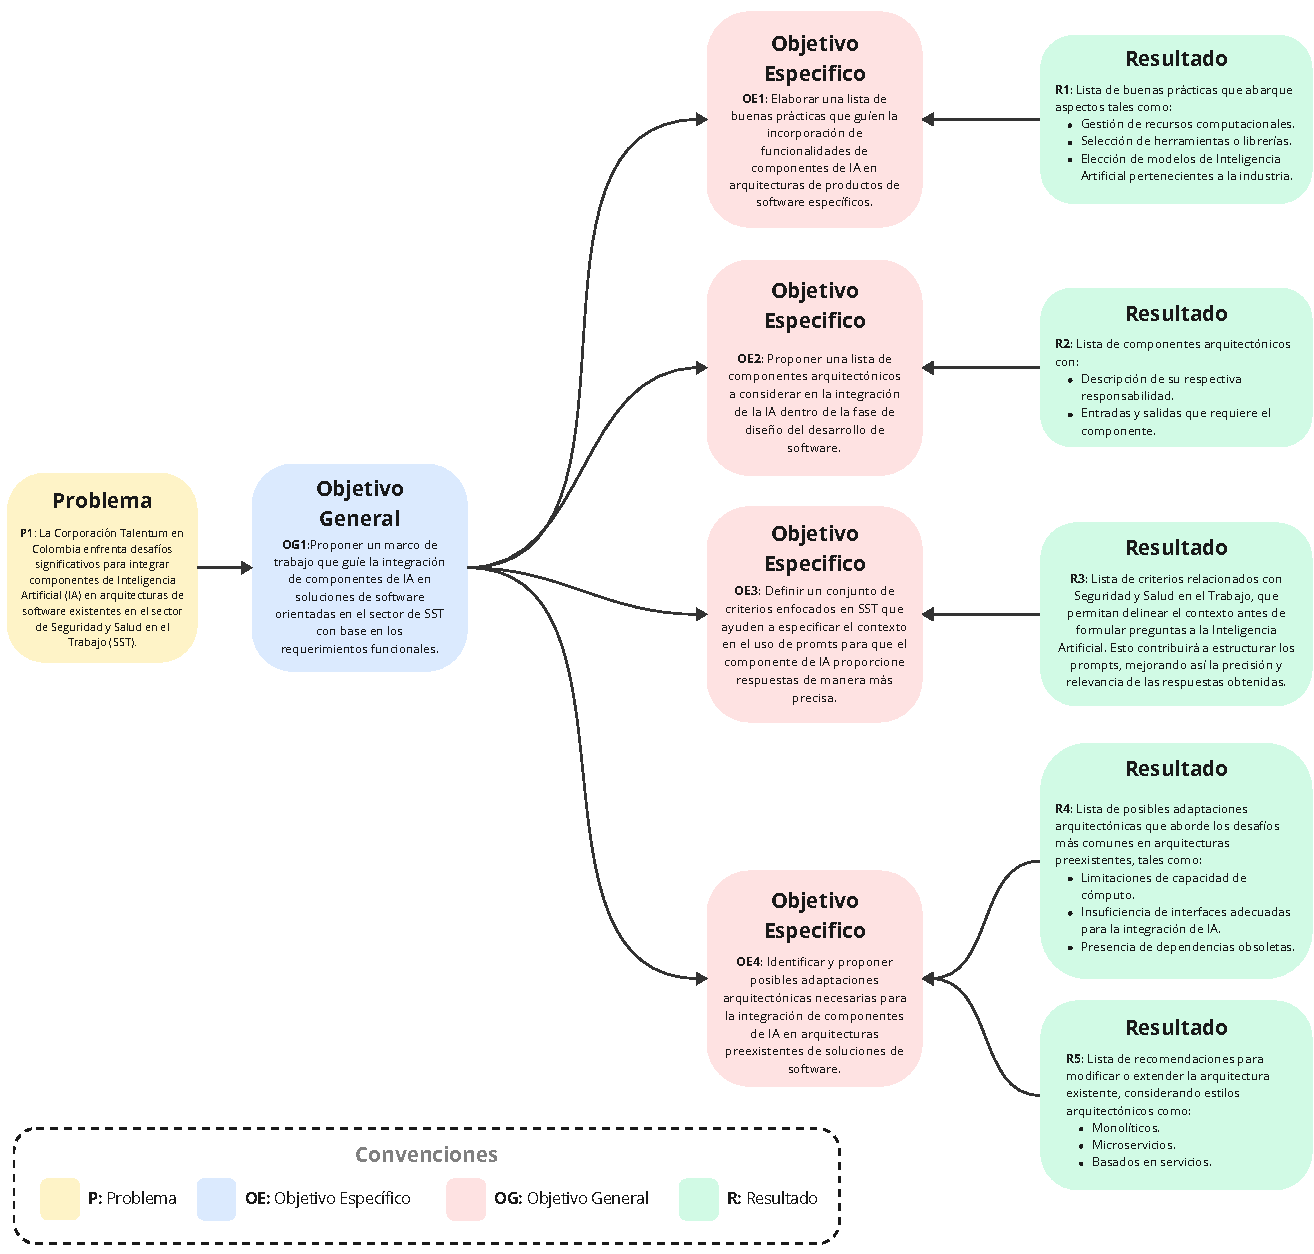
\includegraphics[width=1.15\textwidth]{img/resumen_proyecto.pdf}}
\caption{Diagrama resumen de la propuesta de investigación.}
\label{fig:mi_figura}
\end{figure}